
%{{第二十九回}}{第二十九回}}

\chapter{享福人福深还祷福\hspace{.5em}痴情女情重愈斟情}

{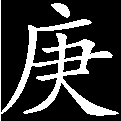
\includegraphics[width=3mm]{../Images/00004} \kaishu 清虚观,贾母、凤姐原意大适意大快乐,偏写出多少不适意事来,此亦天然至情至理必有之事。}

{二玉心事,此回大书,是难了割,却用太君一言以定,是道悉通部书之大旨。}

话说宝玉正自发怔,不想黛玉将手帕子甩了来,正碰在眼睛上,倒唬了一跳,问是谁。林黛玉摇着头儿笑道:``不敢,是我失了手。因为宝姐姐要看呆雁,我比给他看,不想失了手。''宝玉揉着眼睛,待要说什么,又不好说的。

一时,凤姐儿来了,因说起初一日在清虚观打醮的事来,遂约着宝钗、宝玉、黛玉等看戏去。宝钗笑道:``罢,罢,怪热的。什么没看过的戏,我就不去了。''凤姐儿道:``他们那里凉快,两边又有楼。咱们要去,我头几天打发人去,把那些道士都赶出去,把楼打扫干净,挂起帘子来,一个闲人不许放进庙去,才是好呢。我已经回了太太了,你们不去我去。这些日子也闷的很了。家里唱动戏,我又不得舒舒服服的看。''

贾母听说,笑道:``既这么着,我同你去。''凤姐听说,笑道:``老祖宗也去,干净好了!就只是我又不得受用了。''贾母道:``到明儿,我在正面楼上,你在旁边楼上,你也不用到我这边来立规矩,可好不好?''凤姐儿笑道:``这就是老祖宗疼我了。''贾母因又向宝钗道:``你也去,连你母亲也去。长天老日的,在家里也是睡觉。''宝钗只得答应着。

贾母又打发人去请了薛姨妈,顺路告诉王夫人,要带了他们姊妹去。王夫人因一则身上不好,二则预备着元春有人出来,早已回了不去的;听贾母如今这样说,笑道:``还是这么高兴。''因打发人去到园里告诉:``有要逛的,只管初一跟了老太太逛去。''这个话一传开了,别人都还可以,只是那些丫头们天天不得出门槛子,听了这话,谁不要去。便是各人的主子懒怠去,他也百般撺掇了去,因此李宫裁等都说去。贾母越发心中喜欢,早已吩咐人去打扫安置,都不必细说。

单表到了初一这一日,荣国府门前车辆纷纷,人马簇簇。那底下凡执事人等,闻得是贵妃作好事,贾母亲去拈香,正是初一日乃月之首日,况是端阳节间,因此凡动用的什物,一色都是齐全的,不同往日。少时,贾母等出来。贾母坐一乘八人大轿,李氏、凤姐儿、薛姨妈每人一乘四人轿,宝钗、黛玉二人共坐一辆翠盖珠缨八宝车,迎春、探春、惜春三人共坐一辆朱轮华盖车。然后贾母的丫头鸳鸯、鹦鹉、琥珀、珍珠,林黛玉的丫头紫鹃、雪雁、春纤,宝钗的丫头莺儿、文杏,迎春的丫头司棋、绣橘,探春的丫头待书、翠墨,惜春的丫头入画、彩屏,薛姨妈的丫头同喜、同贵,外带着香菱,香菱的丫头臻儿,李氏的丫头素云、碧月,凤姐儿的丫头平儿、丰儿、小红,并王夫人两个丫头也要跟了凤姐儿去的金钏、彩云,奶子抱着大姐儿带着巧姐儿另在一车,还有两个丫头,一共又连上各房的老嬷嬷奶娘并跟出门的家人媳妇子,乌压压的占了一街的车。贾母等已经坐轿去了多远,这门前尚未坐完。这个说``我不同你在一处'',那个说``你压了我们奶奶的包袱'',那边车上又说``蹭了我的花儿'',这边又说``碰折了我的扇子'',咭咭呱呱,说笑不绝。周瑞家的走来过去的说道:``姑娘们,这是街上,看人笑话。''说了两遍,方觉好了。前头的全副执事摆开,早已到了清虚观了。宝玉骑着马,在贾母轿前。街上人都站在两边。

将至观前,只听钟鸣鼓响,早有张法官执香披衣,带领众道士在路旁迎接。贾母的轿刚至山门以内,贾母在轿内因看见有守门大帅并千里眼、顺风耳、当方土地、本境城隍各位泥胎圣像,便命住轿。贾珍带领各子弟上来迎接。凤姐儿知道鸳鸯等在后面,赶不上来搀贾母,自己下了轿,忙要上来搀。可巧有个十二三岁的小道士儿,拿着剪筒,照管剪各处蜡花,正欲得便且藏出去,不想一头撞在凤姐儿怀里。凤姐便一扬手,照脸一下,把那小孩子打了一个筋斗,骂道:``野牛肏的,胡朝那里跑!''那小道士也不顾拾烛剪,爬起来往外还要跑。正值宝钗等下车,众婆娘媳妇正围随的风雨不透,但见一个小道士滚了出来,都喝声叫``拿,拿,拿!打,打,打!''

贾母听了忙问:``是怎么了?''贾珍忙出来问。凤姐上去搀住贾母,就回说:``一个小道士儿,剪灯花的,没躲出去,这会子混钻呢。''贾母听说,忙道:``快带了那孩子来,别唬着他。小门小户的孩子,都是娇生惯养的,那里见的这个势派。倘或唬着他,倒怪可怜见的,他老子娘岂不疼的慌?''说着,便叫贾珍去好生带了来。贾珍只得去拉了那孩子来。那孩子还一手拿着蜡剪,跪在地下乱战。贾母命贾珍拉起来,叫他别怕,问他几岁了。那孩子通说不出话来。贾母还说``可怜见的'',又向贾珍道:``珍哥儿,带他去罢。给他些钱买果子吃,别叫人难为了他。''贾珍答应,领他去了。这里贾母带着众人,一层一层的瞻拜观玩。外面小厮们见贾母等进入二层山门,忽见贾珍领了一个小道士出来,叫人来带去,给他几百钱,不要难为了他。家人听说,忙上来领了下去。

贾珍站在阶矶上,因问:``管家在那里?''底下站的小厮们见问,都一齐喝声说:``叫管家!''登时林之孝一手整理着帽子跑了来,到贾珍跟前。贾珍道:``虽说这里地方大,今儿不承望来这么些人。你使的人,你就带了往你的那院里去;使不着的,打发到那院里去。把小幺儿们多挑几个在这二层门上同两边的角门上,伺候着要东西传话。你可知道不知道,今儿小姐奶奶们都出来,一个闲人也到不了这里。''林之孝忙答应``晓得'',又说了几个``是''。贾珍道:``去罢。''又问:``怎么不见蓉儿?''一声未了,只见贾蓉从钟楼里跑了出来。贾珍道:``你瞧瞧他,我这里也还没敢说热,他倒乘凉去了!''喝命家人啐他。那小厮们都知道贾珍素日的性子,违拗不得,有个小厮便上来向贾蓉脸上啐了一口。贾珍又道:``问着他!''那小厮便问贾蓉道:``爷还不怕热,哥儿怎么先乘凉去了?''贾蓉垂着手,一声不敢说。那贾芸、贾萍、贾芹等听见了,不但他们慌了,亦且连贾璜、贾?、贾琼等也都忙了,一个一个从墙根下慢慢的溜上来。贾珍又向贾蓉道:``你站着作什么?还不骑了马跑到家里,告诉你娘母子去!老太太同姑娘们都来了,叫他们快来伺候。''贾蓉听说,忙跑了出来,一叠声要马,一面抱怨道:``早都不知作什么的,这会子寻趁我。''一面又骂小子:``捆着手呢?马也拉不来。''待要打发小子去,又恐后来对出来,说不得亲自走一趟,骑马去了,不在话下。

且说贾珍方要抽身进去,只见张道士站在旁边陪笑说道:``论理我不比别人,应该里头伺候。只因天气炎热,众位千金都出来了,法官不敢擅入,请爷的示下。恐老太太问,或要随喜那里,我只在这里伺候罢了。''贾珍知道这张道士虽然是当日荣国府国公的替身,曾经先皇御口亲呼为``大幻仙人'',如今现掌``道录司''印,又是当今封为``终了真人'',现今王公藩镇都称他为``神仙'',所以不敢轻慢。二则他又常往两个府里去,凡夫人小姐都是见的。今见他如此说,便笑道:``咱们自己,你又说起这话来。再多说,我把你这胡子还挦了呢!还不跟我进来。''那张道士呵呵大笑,跟了贾珍进来。

贾珍到贾母跟前,控身陪笑说:``这张爷爷进来请安。''贾母听了,忙道:``搀他来。''贾珍忙去搀了过来。那张道士先哈哈笑道:``无量寿佛!老祖宗一向福寿安康?众位奶奶小姐纳福?一向没到府里请安,老太太气色越发好了。''贾母笑道:``老神仙,你好?''张道士笑道:``托老太太万福万寿,小道也还康健。别的倒罢,只记挂着哥儿,一向身上好?前日四月二十六日,我这里做遮天大王的圣诞,人也来的少,东西也很干净,我说请哥儿来逛逛,怎么说不在家?''贾母说道:``果真不在家。''一面回头叫宝玉。谁知宝玉解手去了才来,忙上前问:``张爷爷好?''张道士忙抱住问了好,又向贾母笑道:``哥儿越发发福了。''贾母道:``他外头好,里头弱。又搭着他老子逼着他念书,生生的把个孩子逼出病来了。''张道士道:``前日我在好几处看见哥儿写的字、作的诗,都好的了不得,怎么老爷还抱怨说哥儿不大喜欢念书呢?依小道看来,也就罢了。''又叹道:``我看见哥儿的这个形容身段,言谈举动,怎么就同当日国公爷一个稿子!''说着两眼流下泪来。贾母听说,也由不得满脸泪痕,说道:``正是呢,我养这些儿子孙子,也没一个像他爷爷的,就只这玉儿像他爷爷。''

那张道士又向贾珍道:``当日国公爷的模样儿,爷们一辈的不用说,自然没赶上,大约连大老爷、二老爷也记不清楚了。''说毕呵呵又一大笑,道:``前日在一个人家看见一位小姐,今年十五岁了,生的倒也好个模样儿。我想着哥儿也该寻亲事了。若论这个小姐模样儿,聪明智慧,根基家当,倒也配的过。但不知老太太怎么样,小道也不敢造次。等请了老太太的示下,才敢向人去说。''贾母道:``上回有和尚说了,这孩子命里不该早娶,等再大一大儿再定罢。你可如今打听着,不管他根基富贵,只要模样配的上就好,来告诉我。便是那家子穷,不过给他几两银子罢了。只是模样性格儿难得好的。''

说毕,只见凤姐儿笑道:``张爷爷,我们丫头的寄名符儿你也不换去。前儿亏你还有那么大脸,打发人和我要鹅黄缎子去!要不给你,又恐怕你那老脸上过不去。''张道士呵呵大笑道:``你瞧,我眼花了,也没看见奶奶在这里,也没道多谢。符早已有了,前日原要送去的,不指望娘娘来作好事,就混忘了,还在佛前镇着。待我取来。''说着跑到大殿上去,一时拿了一个茶盘,搭着大红蟒缎经袱子,托出符来。大姐儿的奶子接了符。张道士方欲抱过大姐儿来,只见凤姐笑道:``你就手里拿出来罢了,又用个盘子托着。''张道士道:``手里不干不净的,怎么拿?用盘子洁净些。''凤姐儿笑道:``你只顾拿出盘子来,倒唬我一跳。我不说你是为送符,倒像是和我们化布施来了。''众人听说,哄然一笑,连贾珍也撑不住笑了。贾母回头道:``猴儿猴儿,你不怕下割舌头地狱?''凤姐儿笑道:``我们爷儿们不相干。他怎么常常的说我该积阴骘,迟了就短命呢!''

张道士也笑道:``我拿出盘子来一举两用,却不为化布施,倒要将哥儿的这玉请了下来,托出去给那些远来的道友并徒子徒孙们见识见识。''贾母道:``既这么着,你老人家老天拔地的跑什么,就带他去瞧了,叫他进来,岂不省事?''张道士道:``老太太不知道,看着小道是八十多岁的人,托老太太的福倒也健壮;二则外面的人多,气味难闻,况是个暑热的天,哥儿受不惯,倘或哥儿受了腌臜气味,倒值多了。''贾母听说,便命宝玉摘下通灵玉来,放在盘内。那张道士兢兢业业的用蟒袱子垫着,捧了出去。

这里贾母与众人各处游玩了一回,方去上楼。只见贾珍回说:``张爷爷送了玉来了。''刚说着,只见张道士捧了盘子,走到跟前笑道:``众人托小道的福,见了哥儿的玉,实在可罕。都没什么敬贺之物,这是他们各人传道的法器,都愿意为敬贺之礼。哥儿便不希罕,只留着在房里顽耍赏人罢。''贾母听说,向盘内看时,只见也有金璜,也有玉玦,或有事事如意,或有岁岁平安,皆是珠穿宝贯,玉琢金镂,共有三五十件。因说道:``你也胡闹。他们出家人是那里来的,何必这样,这不能收。''张道士笑道:``这是他们一点敬心,小道也不能阻挡。老太太若不留下,岂不叫他们看着小道微薄,不像是门下出身了。''贾母听如此说,方命人接了。宝玉笑道:``老太太,张爷爷既这么说,又推辞不得,我要这个也无用,不如叫小子们捧了这个,跟着我出去散给穷人罢。''贾母笑道:``这倒说的是。''张道士又忙拦道:``哥儿虽要行好,但这些东西虽说不甚希奇,到底也是几件器皿。若给了乞丐,一则与他们无益,二则反倒遭塌了这些东西。要舍给穷人,何不就散钱与他们。''宝玉听说,便命收下,等晚间拿钱施舍罢了。说毕,张道士方退出去。

这里贾母与众人上了楼,在正面楼上归坐。凤姐等占了东楼。众丫头等在西楼,轮流伺候。贾珍一时来回:``神前拈了戏,头一本《白蛇记》。''贾母问:``《白蛇记》是什么故事?''贾珍道:``是汉高祖斩蛇方起首的故事。第二本是《满床笏》。''贾母笑道:``这倒是第二本上?也罢了。神佛要这样,也只得罢了。''又问第三本,贾珍道:``第三本是《南柯梦》。''贾母听了便不言语。贾珍退了下来,至外边预备着申表、焚钱粮、开戏,不在话下。

且说宝玉在楼上,坐在贾母旁边,因叫个小丫头子捧着方才那一盘子贺物,将自己的玉带上,用手翻弄寻拨,一件一件的挑与贾母看。贾母因看见有个赤金点翠的麒麟,便伸手拿了起来,笑道:``这件东西好像我看见谁家的孩子也带着这么一个的。''宝钗笑道:``史大妹妹有一个,比这个小些。''贾母道:``是云儿有这个。''宝玉道:``他这么往我们家去住着,我也没看见。''探春笑道:``宝姐姐有心,不管什么他都记得。''林黛玉冷笑道:``他在别的上还有限,惟有这些人带的东西上越发留心。''宝钗听说,便回头装没听见。宝玉听见史湘云有这件东西,自己便将那麒麟忙拿起来揣在怀里。一面心里又想到怕人看见他听见史湘云有了,他就留这件,因此手里揣着,却拿眼睛瞟人。只见众人都倒不大理论,惟有林黛玉瞅着他点头儿,似有赞叹之意。宝玉不觉心里没好意思起来,又掏了出来,向黛玉笑道:``这个东西倒好顽,我替你留着,到了家穿上你带。''林黛玉将头一扭,说道:``我不希罕。''宝玉笑道:``你果然不希罕,我少不得就拿着。''说着又揣了起来。

刚要说话,只见贾珍、贾蓉的妻子婆媳两个来了,彼此见过,贾母方说:``你们又来做什么,我不过没事来逛逛。''一句话没说了,只见人报:``冯将军家有人来了。''原来冯紫英家听见贾府在庙里打醮,连忙预备了猪羊香烛茶银之类的东西送礼。凤姐儿听了,忙赶过正楼来,拍手笑道:``嗳呀!我就不防这个。只说咱们娘儿们来闲逛逛,人家只当咱们大摆斋坛的来送礼。都是老太太闹的。这又不得不预备赏封儿。''刚说了,只见冯家的两个管家娘子上楼来了。冯家两个未去,接着赵侍郎也有礼来了。于是接二连三,都听见贾府打醮,女眷都在庙里,凡一应远亲近友,世家相与都来送礼。贾母才后悔起来,说:``又不是什么正经斋事,我们不过闲逛逛,就想不到这礼上,没的惊动了人。''因此虽看了一天戏,至下午便回来了,次日便懒怠去。凤姐又说:``打墙也是动土,已经惊动了人,今儿乐得还去逛逛。''那贾母因昨日张道士提起宝玉说亲的事来,谁知宝玉一日心中不自在,回家来生气,嗔着张道士与他说了亲,口口声声说从今以后不再见张道士了,别人也并不知为什么原故;二则林黛玉昨日回家又中了暑:因此二事,贾母便执意不去了。凤姐见不去,自己带了人去,也不在话下。

且说宝玉因见林黛玉又病了,心里放不下,饭也懒去吃,不时来问。林黛玉又怕他有个好歹,因说道:``你只管看你的戏去,在家里作什么?''宝玉因昨日张道士提亲,心中大不受用,今听见林黛玉如此说,心里因想道:``别人不知道我的心还可恕,连他也奚落起我来。''因此心中更比往日的烦恼加了百倍。若是别人跟前,断不能动这肝火,只是林黛玉说了这话,倒比往日别人说这话不同,由不得立刻沉下脸来,说道:``我白认得了你。罢了,罢了!''林黛玉听说,便冷笑了两声:``我也知道白认得了我,那里像人家有什么配的上呢。''宝玉听了,便向前来直问到脸上:``你这么说,是安心咒我天诛地灭?''林黛玉一时解不过这个话来。宝玉又道:``昨儿还为这个赌了几回咒,今儿你到底又准我一句。我便天诛地灭,你又有什么益处?''林黛玉一闻此言,方想起上日的话来。今日原是自己说错了,又是着急,又是羞愧,便颤颤兢兢的说道:``我要安心咒你,我也天诛地灭。何苦来!我知道,昨日张道士说亲,你怕阻了你的好姻缘,你心里生气,来拿我煞性子。''

原来那宝玉自幼生成有一种下流痴病,况从幼时和黛玉耳鬓厮磨,心情相对;及如今稍明时事,又看了那些邪书僻传,凡远亲近友之家所见的那些闺英闱秀,皆未有稍及林黛玉者,所以早存了一段心事,只不好说出来,故每每或喜或怒,变尽法子暗中试探。那林黛玉偏生也是个有些痴病的,也每用假情试探。因你也将真心真意瞒了起来,只用假意,我也将真心真意瞒了起来,只用假意,如此两假相逢,终有一真。其间琐琐碎碎,难保不有口角之争。即如此刻,宝玉的心内想的是:``别人不知我的心,还有可恕,难道你就不想我的心里眼里只有你!你不能为我烦恼,反来以这话奚落堵我。可见我心里一时一刻白有你,你竟心里没我。''心里这意思,只是口里说不出来。那林黛玉心里想着:``你心里自然有我,虽有`金玉相对'之说,你岂是重这邪说不重我的?我便时常提这`金玉',你只管了然自若无闻的,方见得是待我重,而毫无此心了。如何我只一提`金玉'的事,你就着急,可知你心里时时有`金玉',见我一提,你又怕我多心,故意着急,安心哄我。''

看来两个人原本是一个心,但都多生了枝叶,反弄成两个心了。那宝玉心中又想着:``我不管怎么样都好,只要你随意,我便立刻因你死了也情愿。你知也罢,不知也罢,只由我的心,可见你方和我近,不和我远。''那林黛玉心里又想着:``你只管你,你好我自好,你何必为我而自失。殊不知你失我自失。可见是你不叫我近你,有意叫我远你了。''如此看来,却都是求近之心,反弄成疏远之意。如此之话,皆他二人素习所存私心,也难备述。

如今只述他们外面的形容。那宝玉又听见他说``好姻缘''三个字,越发逆了己意,心里干噎,口里说不出话来,便赌气向颈上抓下通灵宝玉,咬牙恨命往地下一摔,道:``什么捞什骨子,我砸了你完事!''偏生那玉坚硬非常,摔了一下,竟文风没动。宝玉见没摔碎,便回身找东西来砸。林黛玉见他如此,早已哭起来,说道:``何苦来,你摔砸那哑吧物件。有砸他的,不如来砸我。''二人闹着,紫鹃雪雁等忙来解劝。后来见宝玉下死力砸玉,忙上来夺,又夺不下来,见比往日闹的大了,少不得去叫袭人。袭人忙赶了来,才夺了下来。宝玉冷笑道:``我砸我的东西,与你们什么相干!''

袭人见他脸都气黄了,眼眉都变了,从来没气的这样,便拉着他的手,笑道:``你同妹妹拌嘴,不犯着砸他,倘或砸坏了,叫他心里脸上怎么过的去?''林黛玉一行哭着,一行听了这话说到自己心坎儿上来,可见宝玉连袭人不如,越发伤心大哭起来。心里一烦恼,方才吃的香薷饮解暑汤便承受不住,``哇''的一声都吐了出来。紫鹃忙上来用手帕子接住,登时一口一口的把一块手帕子吐湿。雪雁忙上来捶。紫鹃道:``虽然生气,姑娘到底也该保重着些。才吃了药好些,这会子因和宝二爷拌嘴,又吐出来。倘或犯了病,宝二爷怎么过的去呢?''宝玉听了这话说到自己心坎儿上来,可见黛玉不如一紫鹃。又见林黛玉脸红头胀,一行啼哭,一行气凑,一行是泪,一行是汗,不胜怯弱。宝玉见了这般,又自己后悔方才不该同他较证,这会子他这样光景,我又替不了他。心里想着,也由不的滴下泪来了。袭人见他两个哭,由不得守着宝玉也心酸起来,又摸着宝玉的手冰凉,待要劝宝玉不哭罢,一则又恐宝玉有什么委曲闷在心里,二则又恐薄了林黛玉。不如大家一哭,就丢开手了,因此也流下泪来。紫鹃一面收拾了吐的药,一面拿扇子替林黛玉轻轻的扇着,见三个人都鸦雀无声,各人哭各人的,也由不得伤心起来,也拿手帕子擦泪。四个人都无言对泣。

一时,袭人勉强笑向宝玉道:``你不看别的,你看看这玉上穿的穗子,也不该同林姑娘拌嘴。''林黛玉听了,也不顾病,赶来夺过去,顺手抓起一把剪子来要剪。袭人紫鹃刚要夺,已经剪了几段。林黛玉哭道:``我也是白效力。他也不希罕,自有别人替他再穿好的去。''袭人忙接了玉道:``何苦来,这是我才多嘴的不是了。''宝玉向林黛玉道:``你只管剪,我横竖不带他,也没什么。''

只顾里头闹,谁知那些老婆子们见林黛玉大哭大吐,宝玉又砸玉,不知道要闹到什么田地,倘或连累了他们,便一齐往前头回贾母王夫人知道,好不干连了他们。那
贾母王夫人见他们忙忙的作一件正经事来告诉,也都不知有了什么大祸,便一齐进园来瞧他兄妹。急的袭人抱怨紫鹃为什么惊动了老太太、太太,紫鹃又只当是袭人去告诉的,也抱怨袭人。那贾母,王夫人进来,见宝玉也无言,林黛玉也无话,问起来又没为什么事,便将这祸移到袭人紫鹃两个人身上,说:``为什么你们不小心伏侍,这会子闹起来都不管了!''因此将他二人连骂带说教训了一顿。二人都没话,只得听着。还是贾母带出宝玉去了,方才平服。

过了一日,至初三日,乃是薛蟠生日,家里摆酒唱戏,来请贾府诸人。宝玉因得罪了林黛玉,二人总未见面,心中正自后悔,无精打采的,那里还有心肠去看戏,因而推病不去。林黛玉不过前日中了些暑溽之气,本无甚大病,听见他不去,心里想:``他是好吃酒看戏的,今日反不去,自然是因为昨儿气着了。再不然,他见我不去,他也没心肠去。只是昨儿千不该万不该剪了那玉上的穗子。管定他再不带了,还得我穿了他才带。''因而心中十分后悔。

那贾母见他两个都生了气,只说趁今儿那边看戏,他两个见了也就完了,不想又都不去。老人家急的抱怨说:``我这老冤家是那世里的孽障,偏生遇见了这么两个不省事的小冤家,没有一天不叫我操心。真是俗语说的,`不是冤家不聚头'。几时我闭了这眼,断了这口气,凭着这两个冤家闹上天去,我眼不见心不烦,也就罢了。偏又不咽这口气。''自己抱怨着也哭了。

这话传入宝林二人耳内。原来他二人竟是从未听见过``不是冤家不聚头''的这句俗语,如今忽然得了这句话,好似参禅的一般,都低头细嚼此话的滋味,都不觉潸然泣下。虽不曾会面,然一个在潇湘馆临风洒泪,一个在怡红院对月长吁,却不是人居两地,情发一心!

袭人因劝宝玉道:``千万不是,都是你的不是。往日家里小厮们和他们的姊妹拌嘴,或是两口子分争,你听见了,你还骂小厮们蠢,不能体贴女孩儿们的心。今儿你也这么着了。明儿初五,大节下,你们两个再这么仇人似的,老太太越发要生气,一定弄的大家不安生。依我劝,你正经下个气,陪个不是,大家还是照常一样,这么也好,那么也好。''那宝玉听见了不知依与不依,要知端详,且听下回分解。

{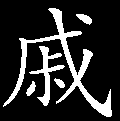
\includegraphics[width=3mm]{../Images/00005}  \kaishu 总评:一片哭声,总因情重;金玉无言,何可为证?}
